%MULTIPLICATION \& DIVISION RELATIONSHIPS - WORKSHEET 0 (IN-CLASS INSTRUCTION)
\documentclass[12pt, letterpaper, fleqn]{article}

% ----------------------------------------------------------
% PACKAGES
% ----------------------------------------------------------
\usepackage{graphicx}
\usepackage{xcolor}
\usepackage[most]{tcolorbox}
\usepackage{amsmath, amssymb}
\usepackage{fancyhdr}
\usepackage[utf8]{inputenc}
\usepackage[T1]{fontenc}
\usepackage{enumitem}
\usepackage{geometry}
\usepackage{tikz}
\usepackage{needspace}
\usepackage{multicol}

\usetikzlibrary{arrows.meta, calc, shapes.geometric}

% ----------------------------------------------------------
% PAGE SETUP
% ----------------------------------------------------------
\usepackage{times}
\geometry{letterpaper, top=1.25in, bottom=1.25in, marginpar=0.5in}

% ----------------------------------------------------------
% HEADER / FOOTER
% ----------------------------------------------------------
\newcommand{\logowidth}{3cm}
\setlength{\headheight}{20pt}
\setlength{\footskip}{40pt}

\pagestyle{fancy}
\fancyhf{}
\fancyhead[C]{\small\bfseries Multiplication \& Division Relationships}
\fancyfoot[L]{\raisebox{2pt}{
\includegraphics[width=\logowidth]{../kss.png}}}
\fancyfoot[C]{\thepage}
\fancyfoot[R]{3.5.0}

\renewcommand{\footrulewidth}{0.2pt}

% ----------------------------------------------------------
% THEME COLOR
% ----------------------------------------------------------
\definecolor{customteal}{HTML}{2fbdb9}

% ----------------------------------------------------------
% HELPER MACROS
% ----------------------------------------------------------
\newcommand{\blank}{\underline{\hspace{2.2cm}}}
\newcommand{\blanklong}{\underline{\hspace{6.5cm}}}
\newcommand{\blankshorter}{\underline{\hspace{1.5cm}}}

% ----------------------------------------------------------
% DOCUMENT
% ----------------------------------------------------------
\begin{document}

\textbf{Name:} \underline{\hspace{5cm}}
\hfill
\textbf{Date:} \underline{\hspace{3cm}}\\

\begin{tcolorbox}[colback=customteal!20]
    \large\textcolor{black}{\textbf{Multiplication & Division Relationships}}
\end{tcolorbox}

\vspace{3mm}
\noindent
Multiplication and division are **opposites** (inverse operations). 
They form **fact families**. For example, 3, 4, and 12 make:
\[
3 \times 4 = 12 \qquad 4 \times 3 = 12
\]
\[
12 \div 3 = 4 \qquad 12 \div 4 = 3
\]

\vspace{3mm}
\begin{center}
\begin{tikzpicture}
\draw[thick, fill=customteal!15] (0,0) -- (1.5, 2.5) -- (3, 0) -- cycle;
\node at (1.5, 2) {\textbf{12}};
\node at (0.4, 0.4) {\textbf{3}};
\node at (2.6, 0.4) {\textbf{4}};
\node at (1.5, -0.4) {Fact Family};
\end{tikzpicture}
\end{center}

\newpage
\begin{tcolorbox}[colback=customteal!20]
    \large\textcolor{black}{\textbf{Guided Practice}}
\end{tcolorbox}

\vspace{5mm}
\noindent
Complete the fact family numbers and write the four equations.

\vspace{8mm}
\begin{enumerate}[itemsep=3cm, leftmargin=0.6cm]
\item Fact Family: \textbf{5, 6, 30}
\begin{itemize}
  \item \blank $\times$ \blank $=$ \blank
  \item \blank $\times$ \blank $=$ \blank
  \item \blank $\div$ \blank $=$ \blank
  \item \blank $\div$ \blank $=$ \blank
\end{itemize}

\item Missing Factor: $4 \times \textsf{?} = 28$. Find the missing factor by writing a division problem.
\\
Division Equation: \blank $\div$ \blank $=$ \blank
\end{enumerate}

\end{document}
